\chapter{机器人运动学与动力学建模}\label{chap:model}

本章先把左右腿等效为可伸缩虚拟杆，建立二维多刚体模型；再针对第二章的混合式闭环连杆机构，给出闭环运动学和任务空间到关节空间的力矩映射；最后将原始广义坐标模型线性化，得到 LQR 控制器所需的状态空间表达式。

\section{建模与基本假设}

若直接用全部连杆和关节变量建立三维模型，模型精度会更高，但维度较大，约束关系也更复杂，不适合直接放入嵌入式控制器中实时计算。结合本文控制系统的规模，本章模型需要完成以下工作：

\begin{enumerate}
  \item 建立二维多刚体模型，描述前进、腿长变化、腿摆和机体俯仰之间的耦合关系；
  \item 给出轮系转角、腿部摆角与控制器状态变量之间的运动学映射；
  \item 推导 LQR 设计所需的线性化状态空间表达式；
  \item 建立闭环腿部机构的任务空间映射，将 VMC 输出转换为关节力矩命令。
\end{enumerate}

建模时保留两套变量：一套是原始广义坐标，用于构造运动控制器的独立坐标模型；另一套是虚拟腿任务空间变量，用于描述腿部支撑和摆动。原始广义坐标取为
\begin{equation}
  \boldsymbol{q} =
  \begin{bmatrix}
    \theta_{wl} & \theta_{wr} & \theta_{ll} & \theta_{lr} & \theta_b
  \end{bmatrix}^{\mathsf{T}}
  \label{eq:generalized-coordinate-origin}
\end{equation}
其中，$\theta_{wl}$ 和 $\theta_{wr}$ 分别表示左、右轮转角，$\theta_{ll}$ 和 $\theta_{lr}$ 分别表示左、右虚拟腿摆角，$\theta_b$ 表示机体俯仰角。与之对应的控制输入记为
\begin{equation}
  \boldsymbol{u} =
  \begin{bmatrix}
    T_{lw,l} & T_{lw,r} & T_{bl,l} & T_{bl,r}
  \end{bmatrix}^{\mathsf{T}}
  \label{eq:input-origin}
\end{equation}
其中，$T_{lw,l}$、$T_{lw,r}$ 为左右轮电机输出转矩，$T_{bl,l}$、$T_{bl,r}$ 为左右腿驱动关节输出转矩。

混合式闭环腿部机构的关节变量耦合较强，直接在关节空间设计支撑和摆动控制并不直观。这里按虚功等效思想，将单腿抽象为连接髋关节与轮轴中心的可伸缩虚拟杆。虚拟杆长度表示腿部伸缩状态，虚拟杆相对竖直方向的转角表示腿部摆动状态。腿部任务空间控制量定义为
\begin{equation}
  \boldsymbol{F}_v =
  \begin{bmatrix}
    F_l \\
    T_\theta
  \end{bmatrix}
  \label{eq:virtual-force-def}
\end{equation}
其中，$F_l$ 为沿虚拟杆方向的轴向虚拟力，用于调节支撑力与腿长；$T_\theta$ 为绕髋关节的虚拟转矩，用于调节腿部摆动姿态。若采用线性弹簧阻尼形式构造虚拟元件，则有
\begin{equation}
  \left\{
    \begin{aligned}
      F_l      &= K_l (l_d - l) + D_l (\dot{l}_d - \dot{l}) \\
      T_\theta &= K_\theta (\theta_{ld} - \theta_l) + D_\theta (\dot{\theta}_{ld} - \dot{\theta}_l)
    \end{aligned}
  \right.
  \label{eq:vmc-law}
\end{equation}
式中，$l_d$ 与 $\theta_{ld}$ 分别为虚拟腿长和平均虚拟腿摆角的期望值；$K_l$、$D_l$、$K_\theta$ 与 $D_\theta$ 分别为对应方向的虚拟刚度系数与虚拟阻尼系数。这样，腿部控制可先在任务空间中给出支撑力和摆动转矩，再映射到实际关节力矩。

为控制模型复杂度，并使模型与后续分层控制器的职责划分一致，本文作如下假设：
\begin{enumerate}
  \item 将机器人简化为机体、左腿、右腿、左驱动轮和右驱动轮五部分组成的刚体系统，忽略连杆柔性变形、轴承间隙和摩擦损失对主要动力学行为的影响；
  \item 忽略腿部闭环连杆机构内部运动产生的附加动力学效应，包括连杆姿态变化、腿长变化和等效惯量变化带来的高阶影响，任一时刻均将腿部视为由当前腿长参数确定的刚体；
  \item 忽略腿部与机体位形变化对驱动轮轴向转动惯量的影响，轮组惯量在建模和控制器设计中取为常值；
  \item 驱动轮与地面满足纯滚动约束，不考虑轮胎侧偏、纵向打滑和接触点弹性变形，后续实验中再结合离地和打滑检测对该假设进行修正；
  \item 机体滚转角由腿部控制器单独补偿，在整机主动力学分析中取滚转角及其一、二阶导数为零，即 $\gamma=\dot{\gamma}=\ddot{\gamma}=0$；
  \item 腿部支撑力由腿部控制器调节，在整机主动力学分析中假设左右腿支撑力保持相等，忽略侧向惯性力矩对运动模型的影响。
\end{enumerate}

上述假设将建模重点集中在前进、俯仰、腿长和腿摆等主要自由度上，同时把滚转补偿、支撑力分配和轮地异常接触留给第四章控制器及第五章实验验证处理。

\section{坐标系与符号定义}

机器人简化刚体模型及坐标系如\figref{fig:model-coordinate} 所示。取地面惯性坐标系 $\Sigma_I = \{O_I, s, h\}$，其中 $s$ 轴沿机器人前进方向，$h$ 轴竖直向上。轮轴中心记为点 $W$，髋关节记为点 $H$，机体质心记为点 $B$。等效虚拟腿长度记为 $l$，平均虚拟腿摆角记为 $\theta_l$，机体俯仰角记为 $\theta_b$，轮半径记为 $R_w$，轮轴中心水平位移记为 $s$。系统偏航角记为 $\phi$，仅在后续状态空间变量构造中使用。

\begin{figure}[H]
  \centering
  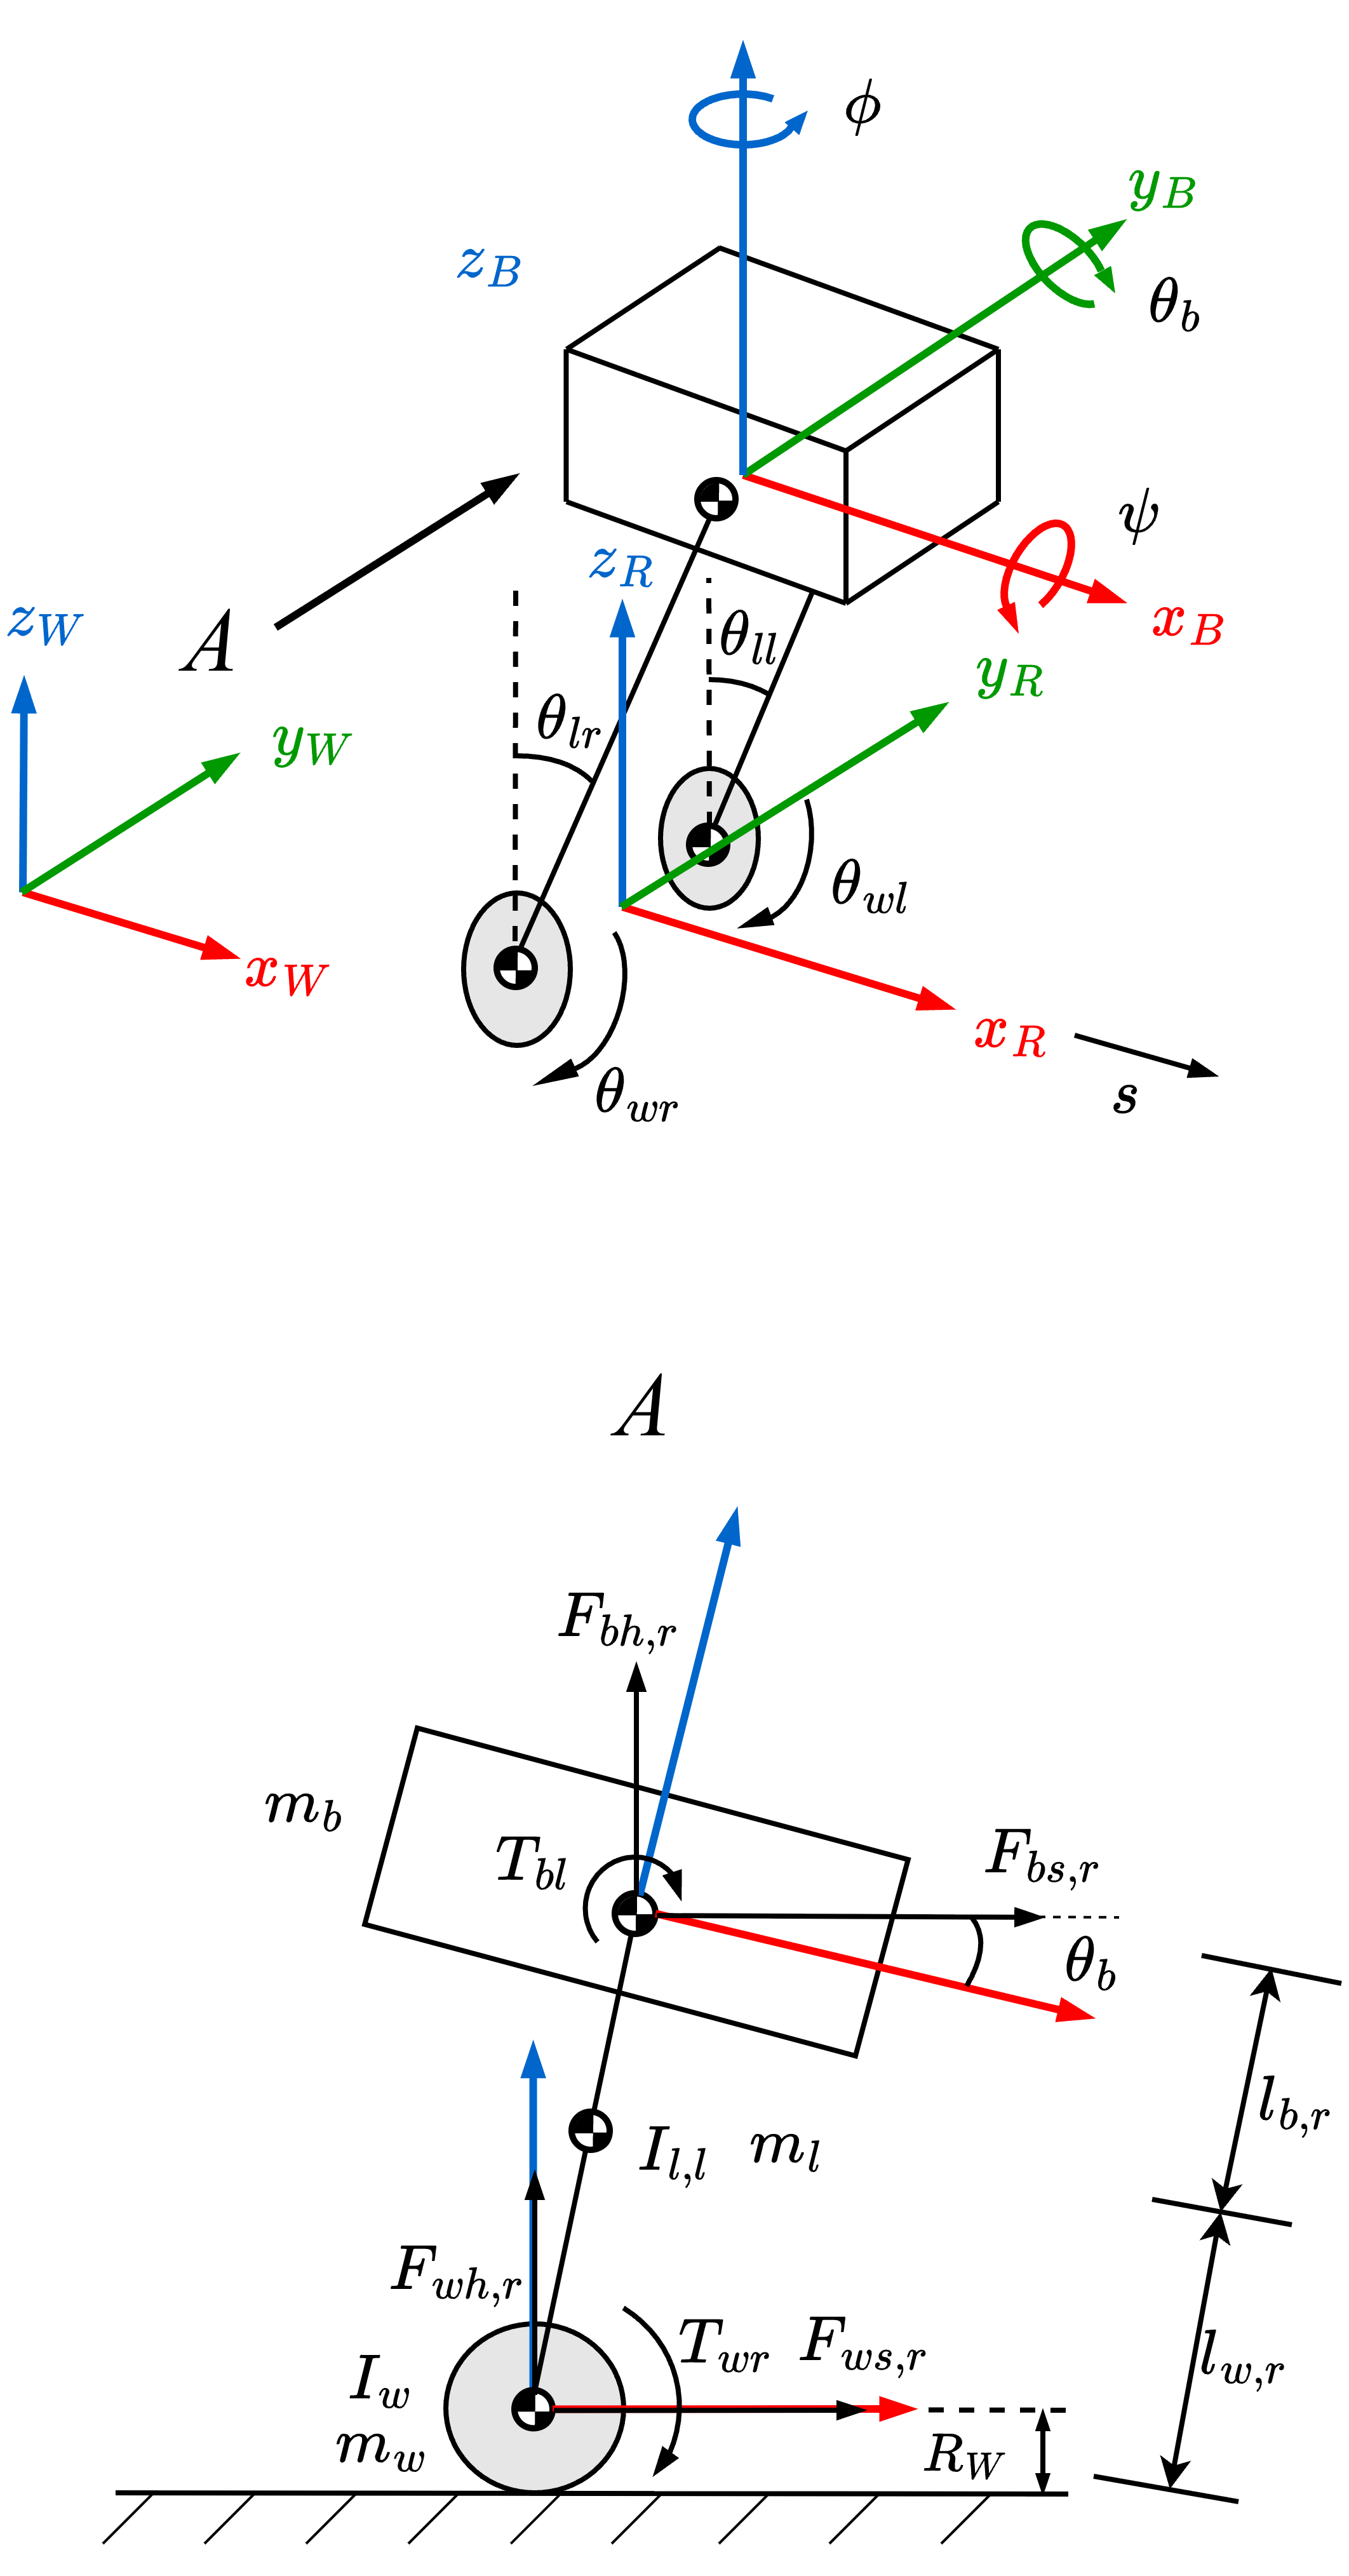
\includegraphics[width=0.48\textwidth]{figures/ch03/robot.png}
  \caption{机器人简化刚体模型及坐标系定义}
  \label{fig:model-coordinate}
\end{figure}

本章主要符号列于\tabref{tab:model-symbols}。

\begin{table}[H]
  \centering
  \caption{模型主要符号定义}\label{tab:model-symbols}
  \renewcommand{\arraystretch}{1.25}
  \begin{tabular}{@{}clp{8.2cm}@{}}
    \toprule
    符号 & 单位 & 含义 \\
    \midrule
    $\theta_{wl} \theta_{wr}$ & rad & 左、右轮转角 \\
    $\theta_{ll} \theta_{lr}$ & rad & 左、右虚拟腿摆角 \\
    $\theta_b$ & rad & 机体俯仰角 \\
    $s$ & m & 轮轴中心在惯性坐标系中的水平位移 \\
    $\phi$ & rad & 机器人偏航角，由左右轮差动及腿部横摆共同决定 \\
    $R_w$ & m & 驱动轮半径 \\
    $R_l$ & m & 半轮距，即机器人纵向中面到单侧轮接地点的距离 \\
    $l_l, l_r$ & m & 左、右腿等效长度参数\\
    $l_b$ & m & 髋关节至机体质心的距离 \\
    $m_w, m_l, m_b$ & kg & 分别表示轮组、虚拟腿等效构件和机体的质量 \\
    $I_w, I_i, I_b$ & kg$\cdot$m$^2$ & 分别表示轮组、虚拟腿等效构件和机体绕质心的转动惯量 \\
    $F_l$ & N & 沿虚拟腿方向的轴向虚拟力 \\
    $T_\theta$ & N$\cdot$m & 绕髋关节作用于虚拟腿的摆动虚拟转矩 \\
    $T_{lw,l} T_{lw,r}$ & N$\cdot$m & 左、右轮电机输出转矩 \\
    $T_{bl,l} T_{bl,r}$ & N$\cdot$m & 左、右腿驱动关节输出转矩 \\
    $\boldsymbol{q}$ & -- & 原始广义坐标向量，取 $\boldsymbol{q} = [\theta_{wl}\, \theta_{wr}\, \theta_{ll}\, \theta_{lr}\, \theta_b]^\mathsf{T}$ \\
    $\boldsymbol{q}_v$ & -- & 二维等效模型广义坐标向量，取 $\boldsymbol{q}_v = [s,\, l,\, \theta_l,\, \theta_b]^\mathsf{T}$ \\
    \bottomrule
  \end{tabular}
\end{table}

\section{多刚体系统运动学建模}

本节建立关键点位置、速度与广义坐标之间的关系。根据\figref{fig:model-coordinate}，分别写出轮轴中心、虚拟腿等效质心、髋关节和机体质心的位置，并由此得到速度和雅可比矩阵。

为避免正文被展开式打断，本节只保留后续控制设计直接使用的运动学关系；左右腿完整位置、速度和加速度方程见附录 \ref{app:kinematics}.

在平面模型下，轮轴中心、虚拟腿等效质心、髋关节和机体质心在惯性坐标系中的位置分别为
\begin{equation}
  \boldsymbol{p}_W =
  \begin{bmatrix}
    s \\
    R_w
  \end{bmatrix}
  \label{eq:w-pos}
\end{equation}
\begin{equation}
  \boldsymbol{p}_L =
  \begin{bmatrix}
    s + \dfrac{l}{2}\sin\theta_l \\
    R_w + \dfrac{l}{2}\cos\theta_l
  \end{bmatrix}
  \label{eq:l-pos}
\end{equation}
\begin{equation}
  \boldsymbol{p}_H =
  \begin{bmatrix}
    s + l\sin\theta_l \\
    R_w + l\cos\theta_l
  \end{bmatrix}
  \label{eq:h-pos}
\end{equation}
\begin{equation}
  \boldsymbol{p}_B =
  \begin{bmatrix}
    s + l\sin\theta_l + l_b\sin\theta_b \\
    R_w + l\cos\theta_l + l_b\cos\theta_b
  \end{bmatrix}.
  \label{eq:b-pos}
\end{equation}
式中，$\boldsymbol{p}_L$、$\boldsymbol{p}_H$ 和 $\boldsymbol{p}_B$ 分别表示虚拟腿等效构件质心、髋关节和机体质心的位置。

由左右轮纯滚动约束可得
\begin{equation}
  s = \frac{R_w}{2}\left(\theta_{wl} + \theta_{wr}\right),\qquad
  \dot{s} = \frac{R_w}{2}\left(\dot{\theta}_{wl} + \dot{\theta}_{wr}\right),\qquad
  \ddot{s} = \frac{R_w}{2}\left(\ddot{\theta}_{wl} + \ddot{\theta}_{wr}\right).
  \label{eq:rolling-constraint}
\end{equation}
\eqref{eq:rolling-constraint} 给出了轮系转角与前进位移之间的几何关系。偏航角不是平面模型中的独立广义坐标，其表达将在第 \ref{sec:state-space-model} 节通过运动学映射引入。

对\eqref{eq:l-pos} 和\eqref{eq:b-pos} 分别对时间求导，可得虚拟腿等效质心和机体质心的速度表达式
\begin{equation}
  \dot{\boldsymbol{p}}_L =
  \begin{bmatrix}
    \dot{s} + \dfrac{\dot{l}}{2}\sin\theta_l + \dfrac{l\dot{\theta}_l}{2}\cos\theta_l \\
    \dfrac{\dot{l}}{2}\cos\theta_l - \dfrac{l\dot{\theta}_l}{2}\sin\theta_l
  \end{bmatrix}
  \label{eq:l-vel}
\end{equation}
\begin{equation}
  \dot{\boldsymbol{p}}_B =
  \begin{bmatrix}
    \dot{s} + \dot{l}\sin\theta_l + l\dot{\theta}_l\cos\theta_l + l_b\dot{\theta}_b\cos\theta_b \\
    \dot{l}\cos\theta_l - l\dot{\theta}_l\sin\theta_l - l_b\dot{\theta}_b\sin\theta_b
  \end{bmatrix}.
  \label{eq:b-vel}
\end{equation}

将\eqref{eq:b-pos} 写成关于等效广义坐标 $\boldsymbol{q}_v$ 的函数形式 $\boldsymbol{p}_B = \boldsymbol{p}_B(\boldsymbol{q}_v)$，则机体质心速度可进一步表示为
\begin{equation}
  \dot{\boldsymbol{p}}_B = \boldsymbol{J}_B(\boldsymbol{q}_v)\dot{\boldsymbol{q}}_v,
  \label{eq:body-jacobian}
\end{equation}
其中，
\begin{equation}
  \boldsymbol{J}_B(\boldsymbol{q}_v) =
  \begin{bmatrix}
    1 & \sin\theta_l & l\cos\theta_l & l_b\cos\theta_b \\
    0 & \cos\theta_l & -l\sin\theta_l & -l_b\sin\theta_b
  \end{bmatrix}.
  \label{eq:body-jacobian-matrix}
\end{equation}

由\eqref{eq:l-vel} 至\eqref{eq:body-jacobian-matrix} 可知，虚拟腿长度 $l$ 与平均腿摆角 $\theta_l$ 不仅决定整机几何构型，也影响机体平动与俯仰运动之间的耦合关系。

\section{多刚体系统动力学建模}

动力学模型用于描述驱动力矩、虚拟腿支撑力和重力作用下的运动响应。平面等效模型由轮组、虚拟腿等效构件和机体三部分组成，下面采用拉格朗日方法建立动力学方程。

系统总动能可写为
\begin{equation}
  T = T_w + T_l + T_b,
  \label{eq:kinetic-total}
\end{equation}
其中
\begin{equation}
  T_w = \frac{1}{2}m_w\dot{s}^2 + \frac{1}{2}I_w\left(\frac{\dot{s}}{R_w}\right)^2,
  \label{eq:kinetic-wheel}
\end{equation}
\begin{equation}
  T_l = \frac{1}{2}m_l \dot{\boldsymbol{p}}_L^\mathsf{T}\dot{\boldsymbol{p}}_L + \frac{1}{2}I_i\dot{\theta}_l^2,
  \label{eq:kinetic-leg}
\end{equation}
\begin{equation}
  T_b = \frac{1}{2}m_b \dot{\boldsymbol{p}}_B^\mathsf{T}\dot{\boldsymbol{p}}_B + \frac{1}{2}I_b\dot{\theta}_b^2.
  \label{eq:kinetic-body}
\end{equation}

取地面为势能零位，则系统总势能为
\begin{equation}
  V = m_l g\left(R_w + \frac{l}{2}\cos\theta_l\right) + m_b g\left(R_w + l\cos\theta_l + l_b\cos\theta_b\right),
  \label{eq:potential-total}
\end{equation}
式中，轮组重力势能为常数项，对动力学方程无影响，因此未单独列出。

引入平面等效广义坐标
\begin{equation}
  \boldsymbol{q}_v =
  \begin{bmatrix}
    s & l & \theta_l & \theta_b
  \end{bmatrix}^{\mathsf{T}}
  \label{eq:generalized-coordinate-v}
\end{equation}
并定义拉格朗日函数
\begin{equation}
  \mathcal{L} = T - V.
  \label{eq:lagrangian}
\end{equation}
则系统满足
\begin{equation}
  \frac{\mathrm{d}}{\mathrm{d}t}\left(\frac{\partial \mathcal{L}}{\partial \dot{\boldsymbol{q}}_v}\right)
  -
  \frac{\partial \mathcal{L}}{\partial \boldsymbol{q}_v}
  = \boldsymbol{Q}_v,
  \label{eq:lagrange-equation}
\end{equation}
其中广义力向量取为
\begin{equation}
  \boldsymbol{Q}_v =
  \begin{bmatrix}
    \dfrac{T_{lw,l} + T_{lw,r}}{2R_w} \\
    F_l \\
    T_\theta \\
    0
  \end{bmatrix}.
  \label{eq:generalized-force}
\end{equation}
式中，第一个分量为左右轮驱动转矩在前进方向上的等效广义力，第二、三项分别对应 VMC 作用下的虚拟腿轴向力与摆动虚拟转矩。机体俯仰自由度不直接受驱动，因此第四项为零。

将\eqref{eq:kinetic-total} 至\eqref{eq:generalized-force} 代入\eqref{eq:lagrange-equation}，可得机器人平面等效模型的动力学方程
\begin{equation}
  \boldsymbol{M}_v(\boldsymbol{q}_v)\ddot{\boldsymbol{q}}_v
  +
  \boldsymbol{C}_v(\boldsymbol{q}_v, \dot{\boldsymbol{q}}_v)\dot{\boldsymbol{q}}_v
  +
  \boldsymbol{G}_v(\boldsymbol{q}_v)
  =
  \boldsymbol{B}_v\boldsymbol{u}_v,
  \label{eq:dynamics-compact}
\end{equation}
其中，
\begin{equation}
  \boldsymbol{u}_v =
  \begin{bmatrix}
    \dfrac{T_{lw,l} + T_{lw,r}}{2} & F_l & T_\theta
  \end{bmatrix}^{\mathsf{T}}\qquad
  \boldsymbol{B}_v =
  \begin{bmatrix}
    1/R_w & 0 & 0 \\
    0 & 1 & 0 \\
    0 & 0 & 1 \\
    0 & 0 & 0
  \end{bmatrix}.
  \label{eq:input-matrix}
\end{equation}

系统质量矩阵 $\boldsymbol{M}_v(\boldsymbol{q}_v)$ 具体为
\begin{equation}
\resizebox{\textwidth}{!}{$
  \boldsymbol{M}_v(\boldsymbol{q}_v) =
  \begin{bmatrix}
    m_w + m_l + m_b + I_w/R_w^2 &
    \left(\dfrac{m_l}{2} + m_b\right)\sin\theta_l &
    \left(\dfrac{m_l}{2} + m_b\right)l\cos\theta_l &
    m_b l_b \cos\theta_b \\
    \left(\dfrac{m_l}{2} + m_b\right)\sin\theta_l &
    \dfrac{m_l}{4} + m_b &
    0 &
    m_b l_b \sin(\theta_l - \theta_b) \\
    \left(\dfrac{m_l}{2} + m_b\right)l\cos\theta_l &
    0 &
    I_i + \dfrac{m_l l^2}{4} + m_b l^2 &
    m_b l l_b \cos(\theta_l - \theta_b) \\
    m_b l_b \cos\theta_b &
    m_b l_b \sin(\theta_l - \theta_b) &
    m_b l l_b \cos(\theta_l - \theta_b) &
    I_b + m_b l_b^2
  \end{bmatrix}
$}
  \label{eq:mass-matrix}
\end{equation}
重力项向量为
\begin{equation}
  \boldsymbol{G}_v(\boldsymbol{q}_v) =
  \begin{bmatrix}
    0 \\
    \left(\dfrac{m_l}{2} + m_b\right) g\cos\theta_l \\
    -\left(\dfrac{m_l}{2} + m_b\right) gl\sin\theta_l \\
    -m_b g l_b \sin\theta_b
  \end{bmatrix}.
  \label{eq:gravity-vector}
\end{equation}
科氏力项和离心力项由矩阵 $\boldsymbol{C}_v(\boldsymbol{q}_v, \dot{\boldsymbol{q}}_v)$ 描述，其元素可由 Christoffel 符号写为
\begin{equation}
  C_{ij} = \frac{1}{2}\sum_{k=1}^{4}
  \left(
    \frac{\partial M_{ij}}{\partial q_k}
    +
    \frac{\partial M_{ik}}{\partial q_j}
    -
    \frac{\partial M_{jk}}{\partial q_i}
  \right)\dot{q}_k.
  \label{eq:christoffel}
\end{equation}

\eqref{eq:dynamics-compact} 中，前进位移、腿长、腿摆和机体俯仰之间的耦合关系已经体现在质量矩阵和重力项中。腿长 $l$ 会改变系统惯性分布和重力项，腿摆角 $\theta_l$ 则通过三角函数项影响机体俯仰耦合。相比直接在关节空间独立处理各驱动量，平面等效模型更便于后续设计分层控制器。

\section{线性化状态空间模型}\label{sec:state-space-model}

前述平面等效模型用于分析整机力学关系和构造任务空间控制量。LQR 控制器还需要标准线性状态空间模型，因此本节回到原始五自由度独立广义坐标，给出线性化过程。

完整受力方程、约束力消元后的线性化方程组以及矩阵 $\boldsymbol{M}$、$\boldsymbol{K}$、$\boldsymbol{E}$ 的展开式见附录 \ref{app:dynamics}. 正文仅保留矩阵形式和状态空间转换关系。

以\eqref{eq:generalized-coordinate-origin} 所示五个独立广义坐标和\eqref{eq:input-origin} 所示四个输入力矩为基础，可用牛顿--欧拉法或拉格朗日法建立原始动力学方程。对轮组、左右腿和机体之间的约束力进行消元后，系统可写成只含独立广义坐标的二阶动力学形式。在直立平衡点附近作小角度近似，并忽略高阶非线性项，可得线性化后的广义动力学方程
\begin{equation}
  \boldsymbol{M}\ddot{\boldsymbol{q}} + \boldsymbol{K}\boldsymbol{q} = \boldsymbol{E}\boldsymbol{u}
  \label{eq:linearized-generalized-model-ch3}
\end{equation}
其中，$\boldsymbol{M}$ 为平衡点处的等效惯性矩阵，$\boldsymbol{K}$ 为线性化后由重力项和耦合项构成的刚度矩阵，$\boldsymbol{E}$ 为输入分配矩阵。由于 $\boldsymbol{M}$ 在工作点附近非奇异，\eqref{eq:linearized-generalized-model-ch3} 可写为
\begin{equation}
  \ddot{\boldsymbol{q}}
  =
  \boldsymbol{A}_{\mathrm{dyn}}\boldsymbol{q}
  +
  \boldsymbol{B}_{\mathrm{dyn}}\boldsymbol{u}
  \qquad
  \boldsymbol{A}_{\mathrm{dyn}} = -\boldsymbol{M}^{-1}\boldsymbol{K}
  \qquad
  \boldsymbol{B}_{\mathrm{dyn}} = \boldsymbol{M}^{-1}\boldsymbol{E}.
  \label{eq:qdd-dyn-ch3}
\end{equation}

\eqref{eq:qdd-dyn-ch3} 给出了广义坐标空间中的加速度表达式。第四章控制器不直接以轮角为状态，而是使用前进位移、偏航角、左右腿摆角和机体俯仰角。因此，还需要建立从广义坐标到控制器状态量的映射。

定义位置状态向量与完整状态向量分别为
\begin{equation}
  \boldsymbol{x}_{\mathrm{pos}}
  =
  \begin{bmatrix}
    s & \phi & \theta_{ll} & \theta_{lr} & \theta_b
  \end{bmatrix}^{\mathsf{T}}
  \label{eq:xpos-ch3}
\end{equation}
\begin{equation}
  \boldsymbol{x}
  =
  \begin{bmatrix}
    s & \dot{s} & \phi & \dot{\phi} & \theta_{ll} & \dot{\theta}_{ll} &
    \theta_{lr} & \dot{\theta}_{lr} & \theta_b & \dot{\theta}_b
  \end{bmatrix}^{\mathsf{T}}.
  \label{eq:state-vector-ch3}
\end{equation}
其中，前进位移 $s$ 已由\eqref{eq:rolling-constraint} 给出。偏航角 $\phi$ 虽不是原始模型中的独立广义坐标，但可由左右轮差动和左右腿摆动的几何关系近似表示为
\begin{equation}
  \phi
  =
  \frac{R_w}{2R_l}\left(-\theta_{wl} + \theta_{wr}\right)
  -
  \frac{l_l}{2R_l}\sin \theta_{ll}
  +
  \frac{l_r}{2R_l}\sin \theta_{lr}.
  \label{eq:yaw-kinematic-map-ch3}
\end{equation}
\eqref{eq:yaw-kinematic-map-ch3} 表明，偏航姿态由轮差动和左右腿摆角共同决定。对该式在直立平衡点附近作小角度线性化，并忽略 $\dot{\theta}^2$ 等高阶项，可得
\begin{equation}
  \ddot{\phi}
  \approx
  \frac{R_w}{2R_l}\left(-\ddot{\theta}_{wl} + \ddot{\theta}_{wr}\right)
  -
  \frac{l_l}{2R_l}\ddot{\theta}_{ll}
  +
  \frac{l_r}{2R_l}\ddot{\theta}_{lr}.
  \label{eq:yaw-acc-linear-ch3}
\end{equation}

定义状态加速度向量
\begin{equation}
  \boldsymbol{x}_{\mathrm{acc}}
  =
  \begin{bmatrix}
    \ddot{s} & \ddot{\phi} & \ddot{\theta}_{ll} & \ddot{\theta}_{lr} & \ddot{\theta}_b
  \end{bmatrix}^{\mathsf{T}}
  \label{eq:xacc-ch3}
\end{equation}
则由\eqref{eq:rolling-constraint} 和\eqref{eq:yaw-acc-linear-ch3} 可得，$\boldsymbol{x}_{\mathrm{acc}}$ 与广义加速度 $\ddot{\boldsymbol{q}}$ 之间满足线性映射
\begin{equation}
  \boldsymbol{x}_{\mathrm{acc}} = \boldsymbol{T}_{\mathrm{map}}\ddot{\boldsymbol{q}}
  \label{eq:tmap-def-ch3}
\end{equation}
其中，
\begin{equation}
  \boldsymbol{T}_{\mathrm{map}}
  =
  \begin{bmatrix}
    \dfrac{R_w}{2} & \dfrac{R_w}{2} & 0 & 0 & 0 \\
    -\dfrac{R_w}{2R_l} & \dfrac{R_w}{2R_l} & -\dfrac{l_l}{2R_l} & \dfrac{l_r}{2R_l} & 0 \\
    0 & 0 & 1 & 0 & 0 \\
    0 & 0 & 0 & 1 & 0 \\
    0 & 0 & 0 & 0 & 1
  \end{bmatrix}.
  \label{eq:tmap-ch3}
\end{equation}

另一方面，在小角度线性化条件下，\eqref{eq:rolling-constraint} 和\eqref{eq:yaw-kinematic-map-ch3} 还可用于将原始广义坐标表示为位置状态的线性组合，即
\begin{equation}
  \boldsymbol{q}
  =
  \boldsymbol{P}\boldsymbol{x}_{\mathrm{pos}}
  \label{eq:q-xpos-map-def-ch3}
\end{equation}
其中，
\begin{equation}
  \boldsymbol{P}
  =
  \begin{bmatrix}
    \dfrac{1}{R_w} & -\dfrac{R_l}{R_w} & -\dfrac{l_l}{2R_w} & \dfrac{l_r}{2R_w} & 0 \\
    \dfrac{1}{R_w} & \dfrac{R_l}{R_w} & \dfrac{l_l}{2R_w} & -\dfrac{l_r}{2R_w} & 0 \\
    0 & 0 & 1 & 0 & 0 \\
    0 & 0 & 0 & 1 & 0 \\
    0 & 0 & 0 & 0 & 1
  \end{bmatrix}.
  \label{eq:q-xpos-map-ch3}
\end{equation}
\eqref{eq:tmap-ch3} 和\eqref{eq:q-xpos-map-ch3} 分别给出了广义加速度到状态加速度、位置状态到广义坐标的映射。

将状态向量\eqref{eq:state-vector-ch3} 按位置与速度两部分分解，可写为
\begin{equation}
  \boldsymbol{x}
  =
  \begin{bmatrix}
    \boldsymbol{x}_{\mathrm{pos}} \\
    \dot{\boldsymbol{x}}_{\mathrm{pos}}
  \end{bmatrix}
  \qquad
  \dot{\boldsymbol{x}}
  =
  \begin{bmatrix}
    \dot{\boldsymbol{x}}_{\mathrm{pos}} \\
    \boldsymbol{x}_{\mathrm{acc}}
  \end{bmatrix}.
  \label{eq:x-split-ch3}
\end{equation}
将\eqref{eq:qdd-dyn-ch3}、\eqref{eq:tmap-def-ch3} 与\eqref{eq:q-xpos-map-def-ch3} 依次联立，可得
\begin{equation}
  \boldsymbol{x}_{\mathrm{acc}}
  =
  \boldsymbol{T}_{\mathrm{map}}
  \left(
    \boldsymbol{A}_{\mathrm{dyn}}\boldsymbol{q}
    +
    \boldsymbol{B}_{\mathrm{dyn}}\boldsymbol{u}
  \right)
  =
  \boldsymbol{T}_{\mathrm{map}}\boldsymbol{A}_{\mathrm{dyn}}\boldsymbol{P}\boldsymbol{x}_{\mathrm{pos}}
  +
  \boldsymbol{T}_{\mathrm{map}}\boldsymbol{B}_{\mathrm{dyn}}\boldsymbol{u}.
  \label{eq:xacc-from-qdd-ch3}
\end{equation}
记
\begin{equation}
  \boldsymbol{A}_p = \boldsymbol{T}_{\mathrm{map}}\boldsymbol{A}_{\mathrm{dyn}}\boldsymbol{P}
  \qquad
  \boldsymbol{B}_p = \boldsymbol{T}_{\mathrm{map}}\boldsymbol{B}_{\mathrm{dyn}}
  \label{eq:ap-bp-ch3}
\end{equation}
则\eqref{eq:x-split-ch3} 可整理为标准连续时间线性状态空间形式
\begin{equation}
  \dot{\boldsymbol{x}}
  =
  \boldsymbol{A}\boldsymbol{x}
  +
  \boldsymbol{B}\boldsymbol{u}
  \label{eq:linear-state-space-ch3}
\end{equation}
其中
\begin{equation}
  \boldsymbol{A}
  =
  \begin{bmatrix}
    \boldsymbol{0}_{5\times5} & \boldsymbol{I}_{5\times5} \\
    \boldsymbol{A}_p & \boldsymbol{0}_{5\times5}
  \end{bmatrix}
  \qquad
  \boldsymbol{B}
  =
  \begin{bmatrix}
    \boldsymbol{0}_{5\times4} \\
    \boldsymbol{B}_p
  \end{bmatrix}.
  \label{eq:ab-matrix-ch3}
\end{equation}

\eqref{eq:linear-state-space-ch3} 至\eqref{eq:ab-matrix-ch3} 给出了从广义动力学方程到状态空间模型的推导过程。这里不展开 $\boldsymbol{A}$、$\boldsymbol{B}$ 的每个元素，而是保留矩阵形式：先在广义坐标空间求加速度，再通过运动学映射转化为控制器状态变量。

\section{腿部机构闭环运动学建模}

前文为整机建模引入了虚拟腿变量，但样机单腿并不是一根实际伸缩杆，而是第二章给出的混合式闭环连杆机构。为使后续控制器能够直接使用腿长 $l$ 与腿部摆角 $\theta_l$，本节先从运动学约束出发证明该混合式机构与标准平面五连杆机构等效，再推导主动关节角到虚拟腿任务空间变量的映射。

腿部机构几何构型见第二章机构简图（\figref{fig:leg-linkage}）。忽略足端轮组自转，并将轮轴中心视为闭链末端汇交点 $P$，则机构的有效运动副由基座两铰点 $A$、$D$、两条主动杆和两条从动杆组成。将两个主动关节角记为 $\theta_{ll}$、$\theta_{lr}$，两个被动关节角记为 $\theta_{pl}$、$\theta_{pr}$。若杆长分别为 $l_1$、$l_2$、$l_3$、$l_4$，则左、右两条支链到达同一末端点 $P$ 的闭环几何约束为
\begin{equation}
  \boldsymbol{p}_A + l_1 \boldsymbol{e}(\theta_{ll}) + l_2 \boldsymbol{e}(\theta_{pl})
  =
  \boldsymbol{p}_D + l_4 \boldsymbol{e}(\theta_{lr}) + l_3 \boldsymbol{e}(\theta_{pr})
  =
  \boldsymbol{p}_P,
  \label{eq:mixed-linkage-loop}
\end{equation}
其中，
\begin{equation}
  \boldsymbol{e}(q) =
  \begin{bmatrix}
    \cos q \\
    \sin q
  \end{bmatrix}.
  \label{eq:unit-vector}
\end{equation}

由\eqref{eq:mixed-linkage-loop} 可见，决定末端点 $P$ 的量只包括基座铰点位置、四根等效杆长、两个主动关节角以及由闭环约束确定的两个被动关节角。混合式结构中用于安装轮组、传动件或加强连接的附加构件，在上述假设下不引入新的独立广义坐标，也不改变 $A$、$D$ 到 $P$ 的闭环矢量方程。因此，对任意给定的主动关节角 $\theta_{ll}$、$\theta_{lr}$，混合式闭环机构与标准平面五连杆机构具有相同的被动关节解、末端位置解和可达工作空间。

若将主动关节向量记为
\begin{equation}
  \boldsymbol{q}_a =
  \begin{bmatrix}
    \theta_{ll} & \theta_{lr}
  \end{bmatrix}^{\mathsf{T}}
  \label{eq:active-joint-vector-ch3}
\end{equation}
则可由闭环约束进一步得到末端速度映射。记
\begin{equation}
  \boldsymbol{E} =
  \begin{bmatrix}
    0 & -1 \\
    1 & 0
  \end{bmatrix}
  \quad
  \boldsymbol{p}_B = \boldsymbol{p}_A + l_1\boldsymbol{e}(\theta_{ll}),
  \quad
  \boldsymbol{p}_C = \boldsymbol{p}_D + l_4\boldsymbol{e}(\theta_{lr}),
  \label{eq:fivebar-intermediate-points}
\end{equation}
其中 $B$、$C$ 分别为左、右主动杆末端。由于从动杆长度保持不变，有
\begin{equation}
  \| \boldsymbol{p}_P - \boldsymbol{p}_B \|^2 = l_2^2,\qquad
  \| \boldsymbol{p}_P - \boldsymbol{p}_C \|^2 = l_3^2.
  \label{eq:passive-link-length-constraint}
\end{equation}
对\eqref{eq:passive-link-length-constraint} 求导，并令
\begin{equation}
  \boldsymbol{u}_l = \frac{\boldsymbol{p}_P-\boldsymbol{p}_B}{l_2}
  \qquad
  \boldsymbol{u}_r = \frac{\boldsymbol{p}_P-\boldsymbol{p}_C}{l_3}
  \label{eq:passive-link-unit-vectors}
\end{equation}
可得
\begin{equation}
  \begin{bmatrix}
    \boldsymbol{u}_l^\mathsf{T} \\
    \boldsymbol{u}_r^\mathsf{T}
  \end{bmatrix}
  \dot{\boldsymbol{p}}_P
  =
  \begin{bmatrix}
    \boldsymbol{u}_l^\mathsf{T} l_1\boldsymbol{E}\boldsymbol{e}(\theta_{ll}) & 0 \\
    0 & \boldsymbol{u}_r^\mathsf{T} l_4\boldsymbol{E}\boldsymbol{e}(\theta_{lr})
  \end{bmatrix}
  \dot{\boldsymbol{q}}_a.
  \label{eq:fivebar-implicit-velocity}
\end{equation}
只要两条从动杆不共线，式中左侧系数矩阵可逆，于是末端点速度可写为
\begin{equation}
  \dot{\boldsymbol{p}}_P = \boldsymbol{J}_P(\boldsymbol{q}_a)\dot{\boldsymbol{q}}_a.
  \label{eq:endpoint-jacobian}
\end{equation}
其中
\begin{equation}
  \boldsymbol{J}_P(\boldsymbol{q}_a)
  =
  \begin{bmatrix}
    \boldsymbol{u}_l^\mathsf{T} \\
    \boldsymbol{u}_r^\mathsf{T}
  \end{bmatrix}^{-1}
  \begin{bmatrix}
    \boldsymbol{u}_l^\mathsf{T} l_1\boldsymbol{E}\boldsymbol{e}(\theta_{ll}) & 0 \\
    0 & \boldsymbol{u}_r^\mathsf{T} l_4\boldsymbol{E}\boldsymbol{e}(\theta_{lr})
  \end{bmatrix}.
  \label{eq:endpoint-jacobian-expression}
\end{equation}
\eqref{eq:endpoint-jacobian-expression} 由闭环长度约束直接求导得到，不需要对包含反三角函数的正运动学解析式再次求偏导，因而更适合嵌入式控制器实时计算。由于该速度雅可比只依赖同一组闭环几何约束，混合式闭环机构与标准五连杆机构还具有相同的末端微分运动学关系。基于上述位置与速度层面的等价性，本文后续将该单腿机构称为等效五连杆机构。

由\eqref{eq:mixed-linkage-loop} 可解得等效五连杆机构末端点 $P$ 的位置 $\boldsymbol{p}_P = [p_s,\ p_h]^\mathsf{T}$，进而定义虚拟腿变量
\begin{equation}
  l = \sqrt{p_s^2 + p_h^2}\qquad
  \theta_l = \operatorname{atan2}(p_s,\, p_h).
  \label{eq:virtual-leg-from-mixed-linkage}
\end{equation}
\eqref{eq:virtual-leg-from-mixed-linkage} 将等效五连杆机构末端位置转换为虚拟腿长度 $l$ 和平均虚拟腿摆角 $\theta_l$。对该式求导，可得
\begin{equation}
  \begin{bmatrix}
    \dot{l} \\
    \dot{\theta}_l
  \end{bmatrix}
  =
  \begin{bmatrix}
    \dfrac{p_s}{l} & \dfrac{p_h}{l} \\
    \dfrac{p_h}{l^2} & -\dfrac{p_s}{l^2}
  \end{bmatrix}
  \dot{\boldsymbol{p}}_P.
  \label{eq:lp-theta-from-p}
\end{equation}

联立\eqref{eq:lp-theta-from-p} 和\eqref{eq:endpoint-jacobian}，得到虚拟腿空间与主动关节空间之间的速度映射
\begin{equation}
  \begin{bmatrix}
    \dot{l} \\
    \dot{\theta}_l
  \end{bmatrix}
  =
  \boldsymbol{J}_v(\boldsymbol{q}_a)\dot{\boldsymbol{q}}_a,
  \qquad
  \boldsymbol{J}_v(\boldsymbol{q}_a) =
  \begin{bmatrix}
    \dfrac{p_s}{l} & \dfrac{p_h}{l} \\
    \dfrac{p_h}{l^2} & -\dfrac{p_s}{l^2}
  \end{bmatrix}
  \boldsymbol{J}_P(\boldsymbol{q}_a).
  \label{eq:virtual-jacobian}
\end{equation}

\eqref{eq:virtual-jacobian} 给出了主动关节速度到虚拟腿任务空间速度的映射。控制系统可由编码器测得的关节角和关节角速度实时计算腿长、腿摆角及其变化率。

\section{腿部机构闭环静力学分析}

闭环运动学关系给出了主动关节空间到虚拟腿任务空间的微分映射。VMC 控制中，腿长方向的支撑力和腿部摆动方向的虚拟转矩并不直接作用在电机轴上，必须通过静力学关系转换为两个主动关节的电机力矩。本节基于虚功原理推导该映射。

设虚拟腿任务空间变量和主动关节力矩分别为
\begin{equation}
  \boldsymbol{x}_v =
  \begin{bmatrix}
    l \\
    \theta_l
  \end{bmatrix}
  \qquad
  \boldsymbol{\tau} =
  \begin{bmatrix}
    \tau_1 \\
    \tau_2
  \end{bmatrix}.
  \label{eq:joint-torque-and-state}
\end{equation}
由\eqref{eq:virtual-jacobian} 可知，任意满足闭环约束的微小虚位移均满足
\begin{equation}
  \delta\boldsymbol{x}_v
  =
  \boldsymbol{J}_v(\boldsymbol{q}_a)\delta\boldsymbol{q}_a.
  \label{eq:virtual-displacement-compatibility}
\end{equation}
若任务空间虚拟广义力为
\begin{equation}
  \boldsymbol{F}_v =
  \begin{bmatrix}
    F_l \\
    T_\theta
  \end{bmatrix}
  \label{eq:virtual-force-vector}
\end{equation}
其中 $F_l$ 为沿虚拟腿方向的轴向力，$T_\theta$ 为绕髋部等效点的虚拟摆动转矩。根据虚功原理，在准静态平衡或忽略惯性项的控制力映射中，关节输入虚功与任务空间虚拟力所作虚功相等，即
\begin{equation}
  \delta W = \boldsymbol{\tau}^\mathsf{T}\delta\boldsymbol{q}_a
  =
  \boldsymbol{F}_v^\mathsf{T}\delta\boldsymbol{x}_v,
  \label{eq:virtual-work}
\end{equation}
将\eqref{eq:virtual-displacement-compatibility} 代入\eqref{eq:virtual-work}，有
\begin{equation}
  \boldsymbol{\tau}^\mathsf{T}\delta\boldsymbol{q}_a
  =
  \boldsymbol{F}_v^\mathsf{T}\boldsymbol{J}_v\delta\boldsymbol{q}_a
  =
  \left(\boldsymbol{J}_v^\mathsf{T}\boldsymbol{F}_v\right)^\mathsf{T}
  \delta\boldsymbol{q}_a.
  \label{eq:virtual-work-substitution}
\end{equation}
由于 $\delta\boldsymbol{q}_a$ 为任意独立虚位移，等式两端关于 $\delta\boldsymbol{q}_a$ 的系数必须相等，因此得到任务空间虚拟力到主动关节力矩的静力学映射
\begin{equation}
  \boldsymbol{\tau} = \boldsymbol{J}_v^\mathsf{T}\boldsymbol{F}_v
  =
  \boldsymbol{J}_v^\mathsf{T}
  \begin{bmatrix}
    F_l \\
    T_\theta
  \end{bmatrix}.
  \label{eq:vmc-torque-map}
\end{equation}

\eqref{eq:vmc-torque-map} 表明，静力学力矩映射由虚拟腿雅可比矩阵的转置给出。对本文腿部机构而言，$F_l$ 主要用于腿长支撑、缓冲与高度调节，$T_\theta$ 主要用于腿部前后摆动和姿态辅助调节。由于 $\boldsymbol{J}_v$ 已由等效五连杆的闭环运动学推导得到，实际控制中只需根据编码器反馈实时更新 $\boldsymbol{J}_v$，即可将 VMC 输出转换为两个主动电机的力矩命令。

若控制器先在末端直角坐标系中生成平面力 $\boldsymbol{F}_P=[F_s,\ F_h]^\mathsf{T}$，也可直接利用末端雅可比矩阵得到
\begin{equation}
  \boldsymbol{\tau}
  =
  \boldsymbol{J}_P^\mathsf{T}(\boldsymbol{q}_a)\boldsymbol{F}_P.
  \label{eq:endpoint-force-torque-map}
\end{equation}
\eqref{eq:vmc-torque-map} 与\eqref{eq:endpoint-force-torque-map} 的本质相同，区别仅在于任务空间坐标选择不同。前者面向腿长与腿摆角控制，便于和第四章 VMC 控制律\eqref{eq:vmc-law} 连接；后者面向末端平面力控制，便于分析轮轴中心受到外力时的关节力矩需求。

\section{本章小结}

本章建立了双轮足机器人的运动学与动力学模型。先给出广义坐标、控制输入和基本假设，将闭环腿部机构等效为可伸缩虚拟杆，并定义 VMC 中的轴向虚拟力 $F_l$ 与摆动虚拟转矩 $T_\theta$。然后建立平面等效模型的坐标系，推导轮轴中心、虚拟腿等效质心、髋关节和机体质心的位置、速度及雅可比表达。在此基础上，采用拉格朗日方法得到多刚体系统动力学方程，并写出质量矩阵、重力项、输入矩阵以及科氏力和离心力项。

之后结合轮系纯滚动约束和偏航运动学近似，推导面向 LQR 控制器的线性状态空间模型。针对五连杆腿部机构，先证明混合式闭环连杆机构与标准五连杆机构在运动学上等效，再建立闭环运动学关系、虚拟腿雅可比矩阵以及基于虚功原理的任务空间到关节空间力矩映射。这些模型将在第四章用于分层控制器设计。
